% !TEX root = ../../t.tex
\chapter{统一交互式的算法可视化网站}
\begin{sectext}
这就是我们截至2012年4月所搭建的算法可视化网站。以下集中讨论的是网站初期阶段,提供的是一些非经典算法的可视化,而不是经典算法的可视化。同时我们将该网站的可视化与网上其他人编写的算法可视化比较,突出其不同之处和我们添加的额外的特点。
\end{sectext}
\section{位掩码、位操作、位串、轻量级布尔值}
\begin{sectext}
整数的位操作(位掩码)对于计算机科学的初学者相对比较微妙。因此,设计一个没有错误的位掩码可视化有助于老师展示不同例子,也有助于学生理解概念。如下面的图所示,例如,$42 | (1 << 2) = 46$。这中基于文本的可视化(如图\ref{fig:1})可以立刻显示必要的位操作。我们现在还没在网上发现其他类似可视化。
% !TEX root = ../../t.tex
\setlength{\belowcaptionskip}{-10pt}
\vspace{-7pt}
\begin{figure}[!htbp]
  \centering
  \frame{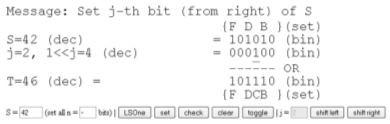
\includegraphics{img/t1}}
  \vspace{-5pt}
  \caption{位掩码的可视化}
  \label{fig:1}
\end{figure}
% \vspace{-10pt}


\end{sectext}
\section{二叉堆(优先队列)}
\begin{sectext}
二叉堆是一种经典的数据结构,通常用于实现优先队列。因特网上有许多其他类似的可视化。在这个可视化中(如图\ref{fig:2}),比起其他的可视化而言,唯一一个优点在于我们的网站拥有统一的风格。
% !TEX root = ../../t.tex
\setlength{\belowcaptionskip}{-10pt}
\vspace{-7pt}
\begin{figure}[!htbp]
  \centering
  \frame{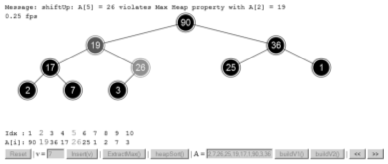
\includegraphics{img/t2}}
  \vspace{-5pt}
  \caption{二叉堆的可视化}
  \label{fig:2}
\end{figure}
% \vspace{-10pt}

\end{sectext}
\section{树状数组}
\begin{sectext}
树状数组由Fenwick(1994)发明。这种数据结构用于高效计算动态区间和查询(RSQ或者累积和频率表),由于在程序竞赛中能发挥奇特的作用,现在已经列入国际信息学奥林匹亚课程的讲解中,参加竞赛的(高中)学生都会学习。树状数组的操作对于初学者可能比较神秘。例如,$RSQ(1, 6)$是$RSQ(1, 4)+RSQ(5, 6)$的和,因为把整数6(二进制表示为``110'')最右边的1截去就变成了4(二进制表示为``100''),再做一次,整数4就变成了0(二进制表示``000''),截到此为止。通过图\ref{fig:3}的动画,这一过程得以清晰展示。我们现在还没在网上发现树状数组的算法可视化。
% !TEX root = ../../t.tex
\setlength{\belowcaptionskip}{-10pt}
\vspace{-7pt}
\begin{figure}[!htbp]
  \centering
  \frame{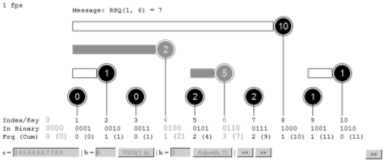
\includegraphics{img/t3}}
  \vspace{-5pt}
  \caption{树状数组的可视化}
  \label{fig:3}
\end{figure}
% \vspace{-10pt}

% !TEX root = ../../t.tex
\setlength{\belowcaptionskip}{-10pt}
\vspace{-7pt}
\begin{figure}[!htbp]
  \centering
  \frame{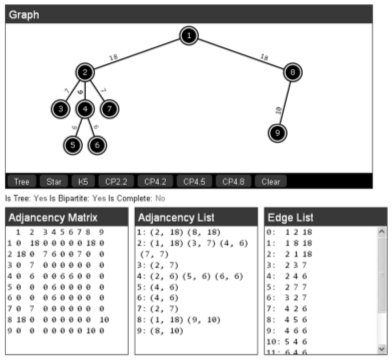
\includegraphics{img/t4}}
  \vspace{-5pt}
  \caption{图数据结构的可视化}
  \label{fig:4}
\end{figure}
% \vspace{-10pt}

\end{sectext}
\section{图}
\begin{sectext}
在网上有许多图的可视化。但是几乎所有的可视化都使用的是内嵌数据的方式,限制了使用方式。我们推测一方面由于难以为输入数据生成图的可视化,另一方面图的布局也是另一个难题。我们提供的可视化支持自定义绘图(如图\ref{fig:4})。自己绘图恰好可以消除我们对于布局算法的考虑。用户也可以添加、删除节点,在节点之间添加边,同时还可以指定方向和权值。用户调整可视化试图的同时,邻接矩阵、临界链表以及边链表也正确地自动更新。还有一个特点在于我们也会判断图的类别,包括树、二分图和完全图。
\end{sectext}
\section{图的遍历:深度优先搜索和广度优先搜索}
\begin{sectext}
在这个可视化中,用户可以像上述内容一样绘制图,然后运行任意一种经典的图遍历算法(DFS或者BFS)。许多关于图遍历的可视化都只实现了这些,但是鉴于这些DFS和BFS算法还包含有额外的关于图结构的信息,于是我们整合进新的特性。对于无向图上的DFS,还可以用Tarjan的算法来计算其强连通分量,如下面的静态图所示(如图\ref{fig:5})。在因特网上,现在也没有网站实现过DFS算法中这两个变量的可视化。对于无权图的BFS,还可以计算从起始点出发的所有最短路径。
% !TEX root = ../../t.tex
\setlength{\belowcaptionskip}{-10pt}
\vspace{-7pt}
\begin{figure}[!htbp]
  \centering
  \frame{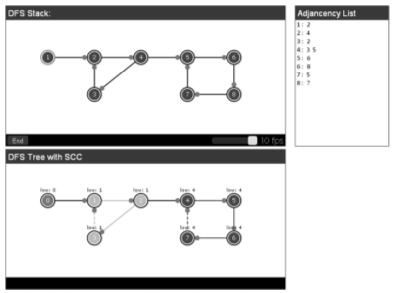
\includegraphics{img/t5}}
  \vspace{-5pt}
  \caption{遍历图的可视化(Tarjan强连通分量/DFS算法)}
  \label{fig:5}
\end{figure}
% \vspace{-10pt}

\end{sectext}
\section{最小生成树(MST):Prim算法和Kruskal算法}
\begin{sectext}
MST算法的可视化确实可以在网上找到,但是下面这个可视化的优势在于用户可以通过绘制图(同时与上述可视化有着相似的用户界面)来了解经典的Prim算法和Kruskal算法在图上的执行。我们还增加额外的功能,把所有边取负后就可以求得最大生成树(如图\ref{fig:6})。
% !TEX root = ../../t.tex
\setlength{\belowcaptionskip}{-1pt}
\vspace{-7pt}
\begin{figure}[!htbp]
  \centering
  \frame{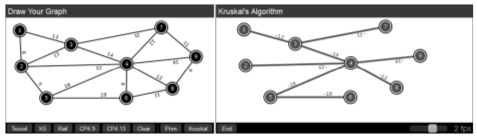
\includegraphics[width=440pt]{img/t6}}
  \vspace{-5pt}
  \caption{MST的可视化(Kruskal算法在用户输入数据的图上执行,其结果中边的权值全部取负)}
  \label{fig:6}
\end{figure}
% \vspace{-10pt}

\end{sectext}
\section{单源最短路径(SSSP):Dijkstra算法和Bellman Ford算法}
\begin{sectext}
SSSP算法的可视化在网上也有很多(特别是Dijkstra算法),但对于使用较少的Bellman Ford算法,其可视化却几乎没有。该算法可视化依然保持一致的用户界面,发挥同样的优势:学生可以自己绘制图。我们还提供SSSP的生成树,方便学生查看最短路径的信息。
% !TEX root = ../../t.tex
\setlength{\belowcaptionskip}{-10pt}
\vspace{-7pt}
\begin{figure}[!htbp]
  \centering
  \frame{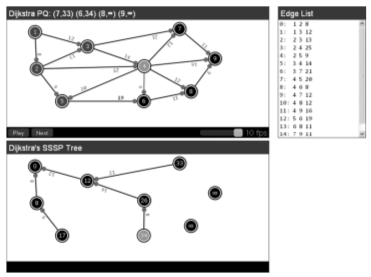
\includegraphics{img/t7}}
  \vspace{-5pt}
  \caption{SSSP的可视化(当源点为1时Dijkstra算法的执行)}
  \label{fig:7}
\end{figure}
% \vspace{-10pt}

\end{sectext}
\section{网络最大流:Edmond Karp算法}
\begin{sectext}
网上网络最大流算法的可视化非常少。我们的可视化(如图\ref{fig:8})有着同样风格的界面,与其他可视化一样也可以自定义图的结构。以后(第五节)我们还会增加不同网络流的模型和变形,加强可视化的效果。
% !TEX root = ../../t.tex
\setlength{\belowcaptionskip}{-1pt}
\vspace{-7pt}
\begin{figure}[!htbp]
  \centering
  \frame{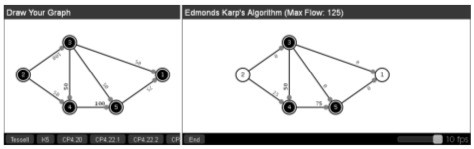
\includegraphics[width=440pt]{img/t8}}
  \vspace{-5pt}
  \caption{最大流的可视化(当源点为2汇点为1时Edmond Karp算法执行的结果)}
  \label{fig:8}
\end{figure}
% \vspace{-10pt}

\end{sectext}
\section{多边形算法:凸包判别、二维凸包}
\begin{sectext}
网上也有一些关于点集中寻找凸包的算法的可视化,但是大部分都是单一可视化。我们的可视化支持三种二维凸包算法:Graham的扫描算法(Graham,1972),如图\ref{fig:9}底部所示,Jarvis的卷包裹算法(Jarvis,1973)以及Andrew的单调链算法(Andrew,1979)。学生在使用这些功能的同时可以比较三种算法在同一个点集上的执行步骤。
% !TEX root = ../../t.tex
\setlength{\belowcaptionskip}{-10pt}
\vspace{-7pt}
\begin{figure}[!htbp]
  \centering
  \frame{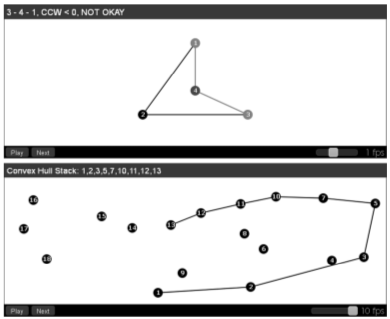
\includegraphics{img/t9}}
  \vspace{-5pt}
  \caption{算法执行过程,其中顶部为凸包判断,底部为Graham扫描算法}
  \label{fig:9}
\end{figure}
% \vspace{-10pt}

另外,对于多边形还有其他许多操作,例如判断任意多边形是凸多边形还是凹多边形(如图\ref{fig:9}顶部)、计算其面积和周长、判断点是否在给定凸多边形或者凹多边形的内部、用直线裁剪多边形。其中一些操作已经在可视化系统中实现,而剩余其他的一些操作将在以后扩展(第五节)。
\end{sectext}
